\chapter{Statistics}

\section{Q1}

  \begin{figure}[H]
    \centering
    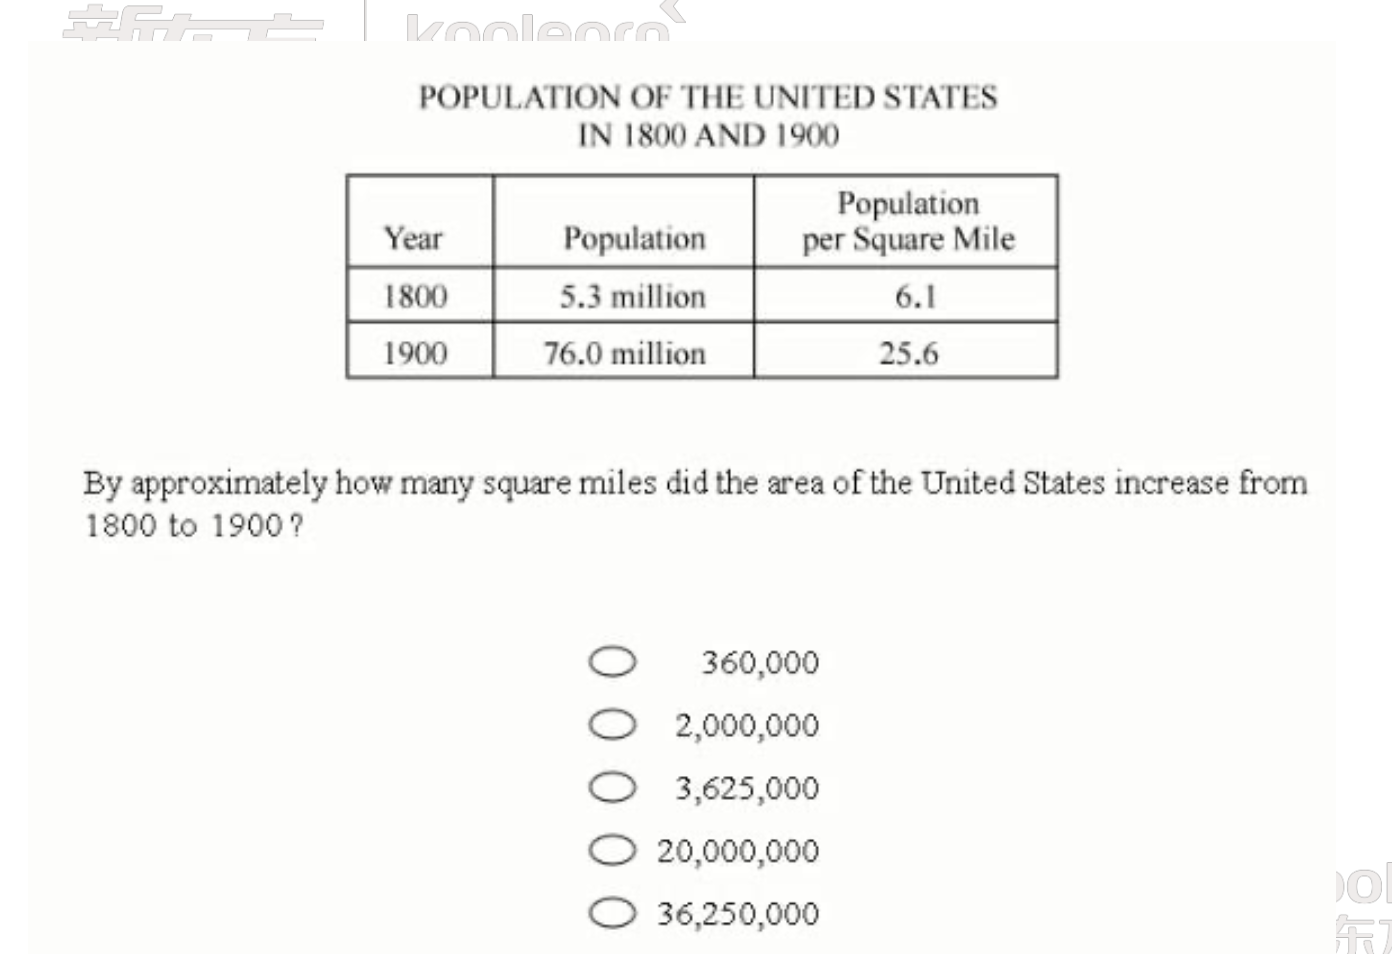
\includegraphics[width=0.7\columnwidth]{images/areas/stats/q1.png}
  \end{figure}

  \subsection{解析}

    \begin{equation*}
      A = \frac{\text{population}}{\text{population per square miles}}
    \end{equation*}

    \textbf{B}

\section{Q2}

  \begin{figure}[H]
    \centering
    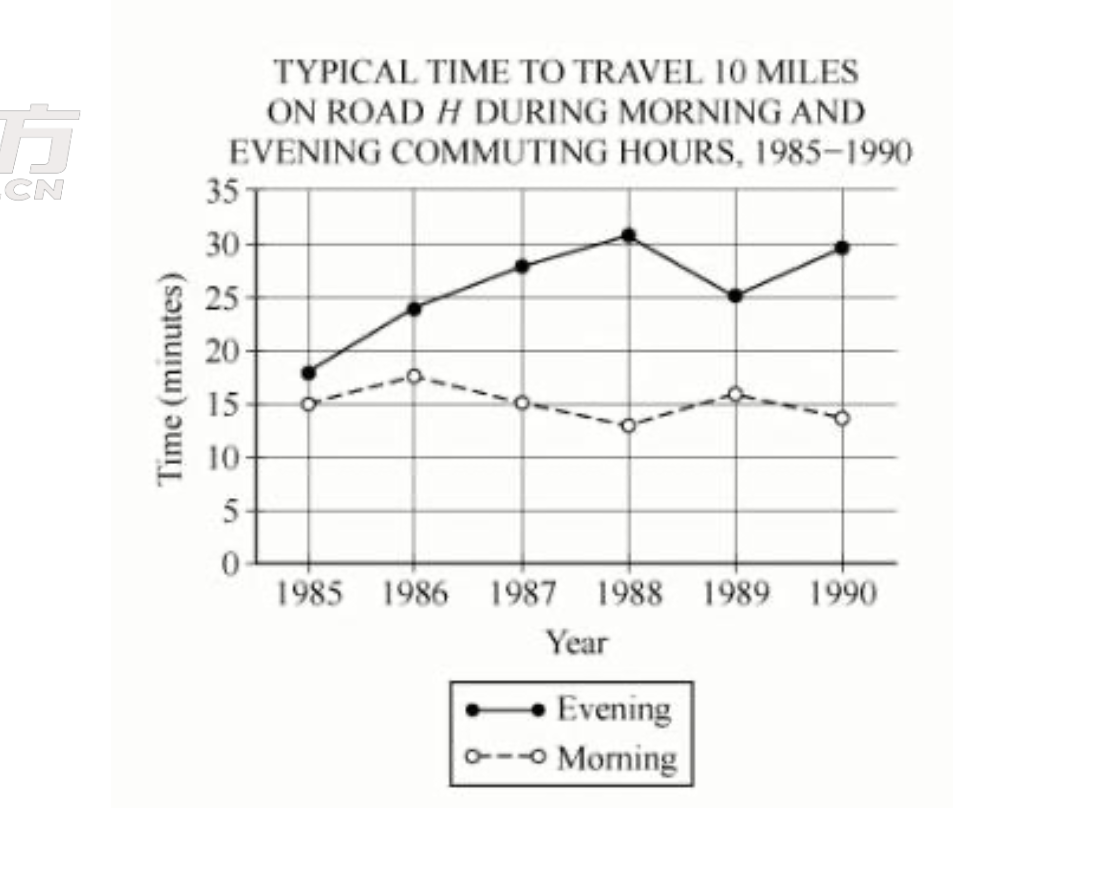
\includegraphics[width=0.7\columnwidth]{images/areas/stats/q2.png}
  \end{figure}

  The typical travel time during the morning commuting hours decreased by
  approximately what percent from 1986 to 1998?

  \begin{enumerate}
    \item 5\%
    \item 10\%
    \item 25\%
    \item 40\%
    \item 45\%
  \end{enumerate}

  \subsection{解析}

    \textbf{C}: 这种题要通过约分来做, 约分后1986年是20, 1988年是15. 所以下降百分之25

\section{Q3}

  Martha invited 4 friends to go with her to the movies. There are 120
  different ways in which they can sit together in a row of 5 seats,
  one person per seat. In how many of those ways is Martha sitting in the
  middle seat?

  \subsection{解析}

    Martha坐中间, 所以先让Martha做

    \begin{equation*}
      4 \times 3 \times 2 \times 1 = 24
    \end{equation*}

\section{Q4}

  From a box of 10 light bulbs, you are to remove 4. How many different sets
  of 4 light bulbs could you remove?

  \subsection{解析}

    \begin{align*}
      n &= 10 \\
      r &= 4 \\
      s &= \frac{10!}{4!\left( 10 - 4 \right)!} \\
      &= 210
    \end{align*}

\section{Q5}

  In a box of 10 electrical parts, 2 are defective.

  \begin{enumerate}
    \item If you choose one part at random from the box, what is the
    probability that it is not defective?
    \item If you choose two parts at random from the box, without replacement,
    what is the probability that both are defective?
  \end{enumerate}

  \subsection{解析}

    \begin{enumerate}
      \item $ \frac{4}{5} $
      \item $ \frac{1}{45} $
    \end{enumerate}

\section{Q6}

  Lin and Mark each attempt independently to decode a message.
  If the probability that Lin will decode the message is 0.80 and the
  probability that Mark will decode the message is 0.70,
  find the probability that

  \begin{enumerate}
    \item at least one of them will decode the message
  \end{enumerate}

  \subsection{解析}

    都没找到的可能性是

    \begin{equation*}
      \left( 1 - 0.8 \right) \times \left( 1 - 0.7 \right) = 0.06
    \end{equation*}

    只要一个人找到是都没找到的反面, 所以

    \begin{equation*}
      1 - 0.06 = 0.94
    \end{equation*}
